%!TEX program = xelatex
% Encoding: UTF8
% SEIKA 2015

%\documentclass[a4paper,11pt,twoside]{article}
\documentclass[a4paper,11pt,twoside]{ctexart}

% 支持西文字体
\usepackage{fourier}

\usepackage{geometry}
\geometry{left=3.5cm, right=3cm, top=3.cm, bottom=3cm}
%控制页眉页脚页码
\pagestyle{headings}
%罗马字符页码
%\pagenumbering{roman}

%\usepackage{ctex}    uncomment this if article is applied on docclass
%\usepackage{xeCJK}   uncomment this if article is applied on docclass

%\CJKsetecglue{} % 禁用汉字与其他内容之间空格(空隙)
%\usepackage{ctex}

\usepackage{graphicx}
% 支持插入eps图形文件
\usepackage{epsfig}

% 支持超链接
\usepackage[colorlinks]{hyperref}

% 插入
\usepackage{listings}
\usepackage{xcolor}

% \setCJKmainfont[BoldFont={SimSun},ItalicFont={KaiTi}] %{SimSun}
%%%%%%%%%%%%
\title{Tensorflow 指南}
\author{}
\date{2015-12-16}
% \thanks{}

\begin{document}

\maketitle
\newpage
\tableofcontents
\newpage

\section{起步}

\section{基础教程}
\subsection {综述}

\subsection {MNIST之机器学习入门}

This tutorial is intended for readers who are new to both machine learning and TensorFlow. If you already know what MNIST is, and what softmax (multinomial logistic) regression is, you might prefer this faster paced tutorial. Be sure to install TensorFlow before starting either tutorial.

这个教程的目标读者是对机器学习和TensorFlow都不太了解的新手。如果你已经了解MNIST和softmax回归(softmax regression)的相关知识,你可以阅读这个快速上手教程。

When one learns how to program, there's a tradition that the first thing you do is print "Hello World." Just like programming has Hello World, machine learning has MNIST.

当我们开始学习编程的时候,第一件事往往是学习打印“Hello World”。就好比编程入门有Hello World,机器学习入门有MNIST。
MNIST是一个入门级的计算机视觉数据集,它包含各种手写数字图片:

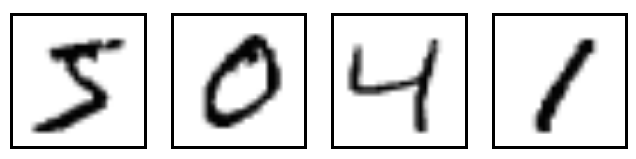
\includegraphics[width=.8\textwidth]{../SOURCE/images/MNIST.png}

它也包含每一张图片对应的标签,告诉我们这个是数字几。比如,上面这四张图片的标签分别是5,0,4,1。
在此教程中,我们将训练一个机器学习模型用于预测图片里面的数字。我们的目的不是要设计一个世界一流的复杂模型 -- 尽管我们会在之后给你源代码去实现一流的预测模型 -- 而是要介绍下如何使用TensorFlow。所以,我们这里会从一个很简单的数学模型开始,它叫做Softmax Regression。
对应这个教程的实现代码很短,而且真正有意思的内容只包含在三行代码里面。但是,去理解包含在这些代码里面的设计思想是非常重要的:TensorFlow工作流程和机器学习的基本概念。因此,这个教程会很详细地介绍这些代码的实现原理。

\subsubsection {MNIST数据集}

MNIST数据集的官网是\href{http://yann.lecun.com/exdb/mnist/}{Yann LeCun's website}。在这里,我们提供了一份python源代码用于自动下载和安装这个数据集。你可以下载这段\href{https://tensorflow.googlesource.com/tensorflow/+/master/tensorflow/examples/tutorials/mnist/input_data.py}{代码},然后用下面的代码导入到你的项目里面,也可以直接复制粘贴到你的代码文件里面。

\begin{colorboxed}
  \begin{lstlisting}[language={[ANSI]Python}, numbers=left,numberstyle=\tiny,
      frame=shadowbox, rulesepcolor=\color{red!20!green!20!blue!20},
      keywordstyle=\color{blue!70!black},
      commentstyle=\color{blue!90!},
      basicstyle=\ttfamily]
import input_data
mnist = input_data.read_data_sets("MNIST_data/", one_hot=True)
  \end{lstlisting}
\end{colorboxed}

下载下来的数据集被分成两部分:60000行的训练数据集(`mnist.train`)和10000行的测试数据集(`mnist.test`)。这样的切分很重要,在机器学习模型设计时必须有一个单独的测试数据集不用于训练而是用来评估这个模型的性能,从而更加容易把设计的模型推广到其他数据集上(泛化)。

正如前面提到的一样,每一个MNIST数据单元有两部分组成:一张包含手写数字的图片和一个对应的标签。我们把这些图片设为“xs”,把这些标签设为“ys”。训练数据集和测试数据集都包含xs和ys,比如训练数据集的图片是 `mnist.train.images` ,训练数据集的标签是 `mnist.train.labels`。

每一张图片包含$ 28 \times 28$像素。我们可以用一个数字数组来表示这张图片:

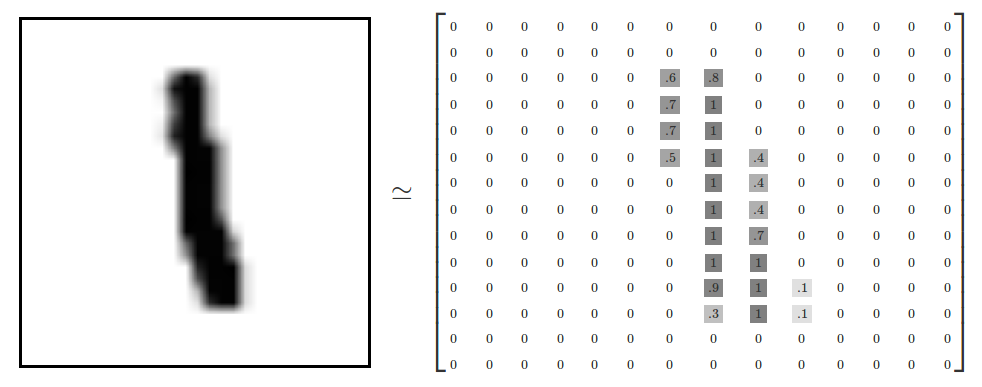
\includegraphics[width=.85\textwidth]{../SOURCE/images/MNIST-Matrix.png}

我们把这个数组展开成一个向量,长度是 $ 28 \times 28 = 784$。如何展开这个数组(数字间的顺序)不重要,只要保持各个图片采用相同的方式展开。从这个角度来看,MNIST数据集的图片就是在784维向量空间里面的点, 并且拥有比较复杂的结构 (提醒: 此类数据的可视化是计算密集型的)。

展平图片的数字数组会丢失图片的二维结构信息。这显然是不理想的,最优秀的计算机视觉方法会挖掘并利用这些结构信息,我们会在后续教程中介绍。但是在这个教程中我们忽略这些结构,所介绍的简单数学模型,softmax回归(softmax regression),不会利用这些结构信息。

因此,在MNIST训练数据集中,mnist.train.images 是一个形状为 [60000, 784] 的张量,第一个维度数字用来索引图片,第二个维度数字用来索引每张图片中的像素点。在此张量里的每一个元素,都表示某张图片里的某个像素的强度值,值介于0和1之间。

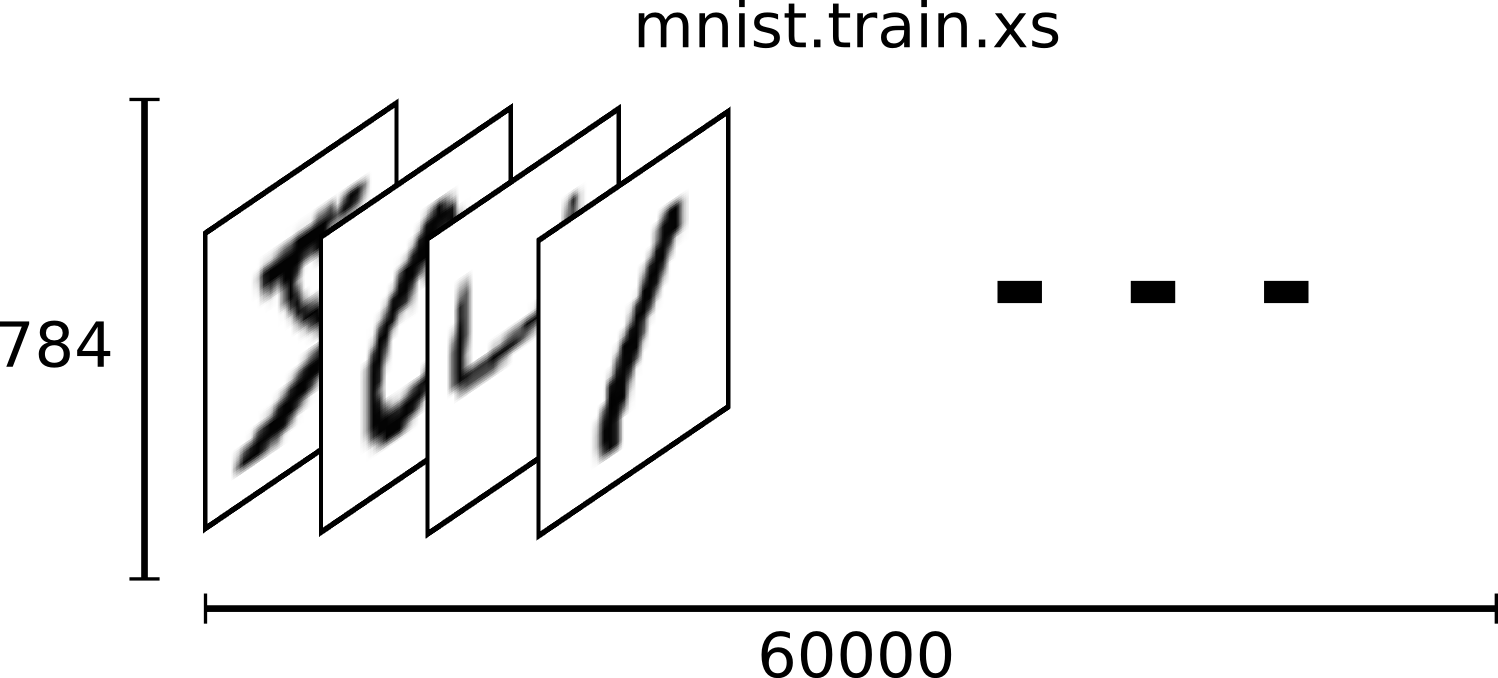
\includegraphics[width=.75\textwidth]{../SOURCE/images/mnist-train-xs.png}

相对应的MNIST数据集的标签是介于0到9的数字,用来描述给定图片里表示的数字。为了用于这个教程,我们使标签数据是"one-hot vectors"。 一个one-hot向量除了某一位的数字是1以外其余各维度数字都是0。所以在此教程中,数字n将表示成一个只有在第n维度(从0开始)数字为1的10维向量。比如,标签0将表示成([1,0,0,0,0,0,0,0,0,0,0])。因此, mnist.train.labels 是一个 [60000, 10] 的数字矩阵。

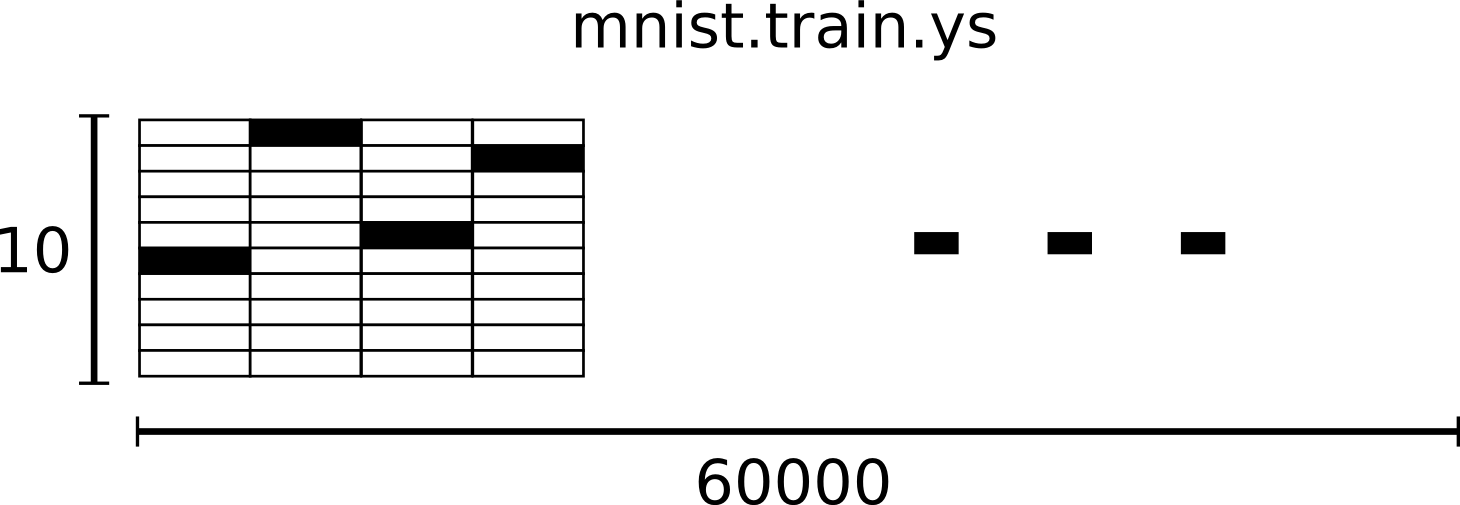
\includegraphics[width=.75\textwidth]{../SOURCE/images/mnist-train-ys.png}

现在,我们准备开始真正的建模之旅啦!

\subsubsection {Softmax回归介绍}

我们知道MNIST的每一张图片都表示一个数字,从0到9。我们希望得到给定图片代表每个数字的概率。比如说,我们的模型可能推测一张包含9的图片代表数字9的概率是80\%但是判断它是8的概率是5\%(因为8和9都有上半部分的小圆),然后给予它代表其他数字的概率更小的值。

这是一个使用softmax回归(softmax regression)模型的经典案例。softmax模型可以用来给不同的对象分配概率。即使在之后,我们训练更加精细的模型时,最后一步也需要用softmax来分配概率。

softmax回归(softmax regression)分两步:第一步

为了得到一张给定图片属于某个特定数字类的证据(evidence),我们对图片像素值进行加权求和。如果这个像素具有很强的证据说明这张图片不属于该类,那么相应的权值为负数,相反如果这个像素拥有有利的证据支持这张图片属于这个类,那么权值是正数。
下面的图片显示了一个模型学习到的图片上每个像素对于特定数字类的权值。红色代表负数权值,蓝色代表正数权值。


\section{TensorFlow运作方式}

\subsection {本教程使用文件}
\subsection {准备数据}
\subsection {构建图表}
\subsection {模型训练}
\subsection {模型评估}
\subsection {模型评估}

\section{卷积神经网络}
\subsection {概述}
\subsection {代码组织}
\subsection {CIFAR-10模型}
\subsection {开始执行并训练模型}
\subsection {模型评估}



\section{其他}

\end{document}